	\begin{figure}[!ht]
		\label{venn_diagram}

		\centering

		\def\loclb{(180:2.0cm) circle (2.0cm)}
	  	\def\loclf{(0:2.0cm) circle (2.0cm)}
	  	\def\locrb{(90:2.0cm) circle (2.0cm)}
	  	\def\locrf{(270:2.0cm) circle (2.0cm)}

      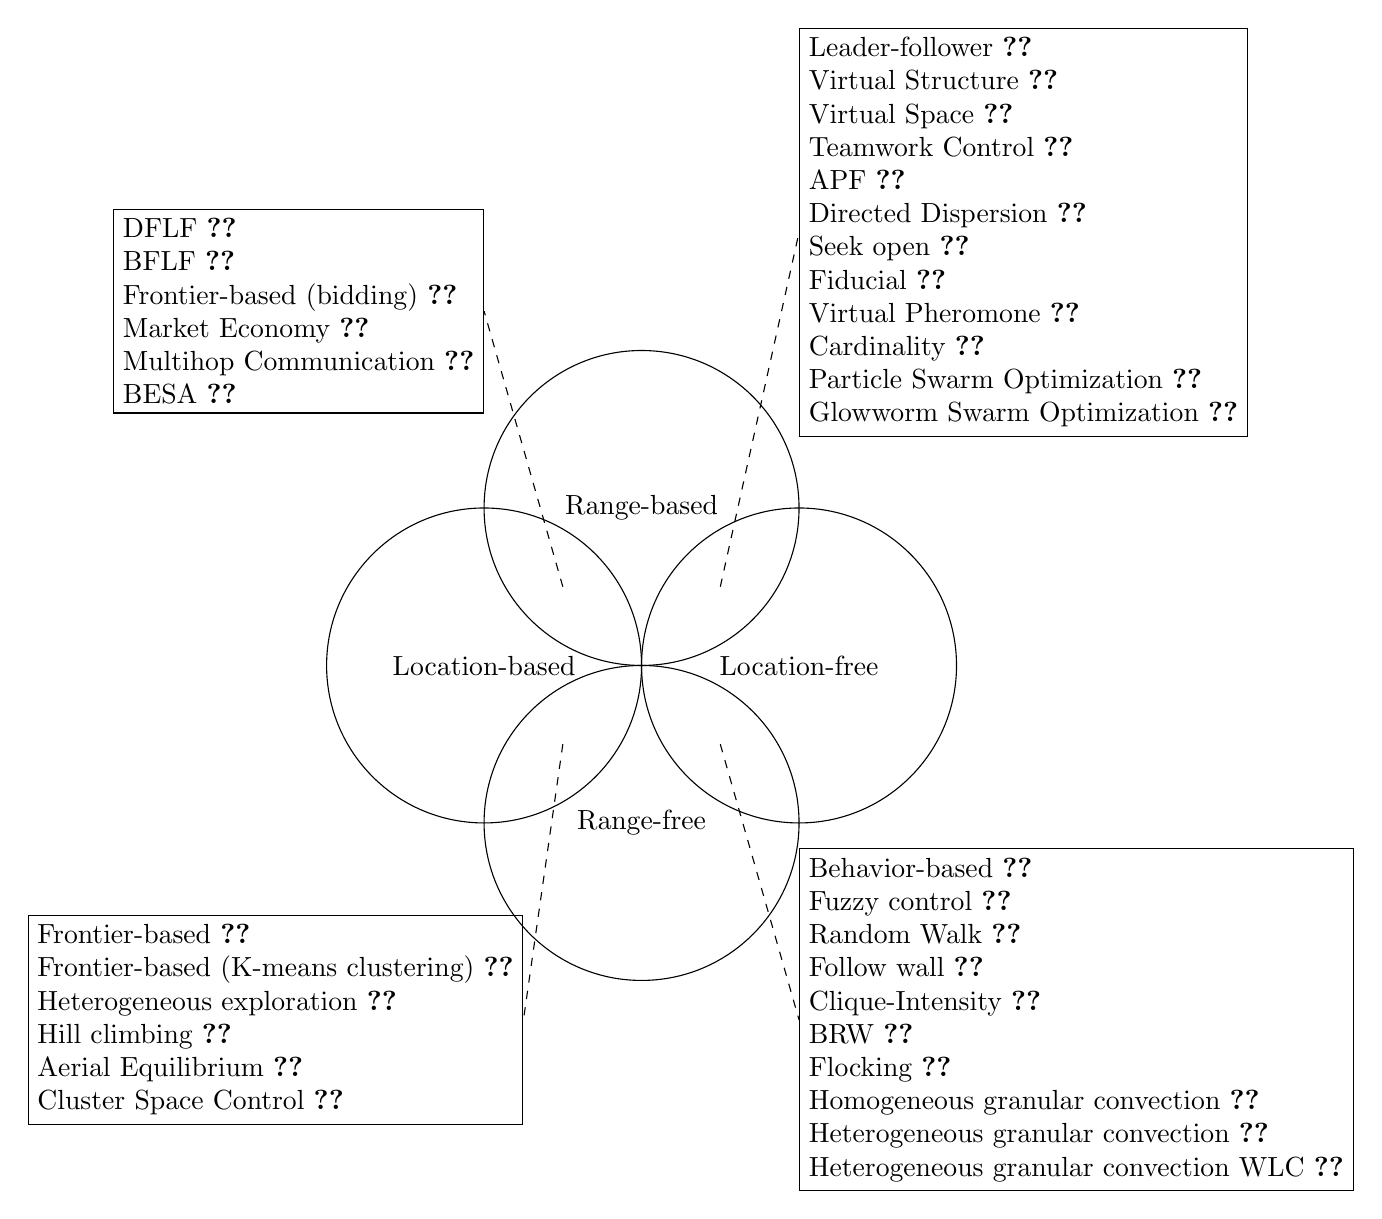
\begin{tikzpicture}%[thick,scale=0.8, every node/.style={scale=0.8}]
			% standard figures
			\draw \loclb node [text=black] {Location-based};
			\draw \loclf node [text=black] {Location-free};
			\draw \locrb node [text=black] {Range-based};
			\draw \locrf node [text=black] {Range-free};

			% Range-based location-free
			\draw[dashed,-] (1,1) -- (2,5.5) node[anchor=north west] {};
			\node[draw,align=left,anchor=west] at (2,5.5) {
				Leader-follower \ref{sec:Formation}\\
				Virtual Structure \ref{sec:Formation}\\
				Virtual Space \ref{sec:Formation}\\
				Teamwork Control \ref{sec:Formation}\\
				APF \ref{sec:Dispersion}\\
				Directed Dispersion \ref{sec:Dispersion}\\
				Seek open \ref{sec:Dispersion}\\
				Fiducial \ref{sec:Dispersion}\\
				Virtual Pheromone \ref{sec:Exploration}\\
				Cardinality \ref{sec:Exploration}\\
				Particle Swarm Optimization \ref{sec:Localization}\\
				Glowworm Swarm Optimization \ref{sec:Localization}
			};

			% Range-free, location-free
			\draw[dashed,-] (1,-1) -- (2,-4.5) node[anchor=north west] {};
			\node[draw,align=left,anchor=west] at (2,-4.5) {
				Behavior-based \ref{sec:Formation}\\
				Fuzzy control \ref{sec:Formation}\\
				Random Walk \ref{sec:Dispersion}\\
				Follow wall \ref{sec:Dispersion}\\
				Clique-Intensity \ref{sec:Dispersion}\\
				BRW \ref{sec:Exploration}\\
				Flocking \ref{sec:CollectiveTransport}\\
				Homogeneous granular convection \ref{sec:CollectiveTransport}\\
				Heterogeneous granular convection \ref{sec:CollectiveTransport}\\
				Heterogeneous granular convection WLC \ref{sec:CollectiveTransport}
				%Virtual Pheromone \ref{sec:Path-planning}\\
				%Cardinality \ref{sec:Path-planning}
			};

			% % location-free
			% \draw[dashed,-] (3.5,0) -- (4.3,0) node[anchor=north west] {};
			% \node[draw,align=left,anchor=west] at (4.3,0) {
			% 	Biased Random Walk \ref{sec:Localization}
			% };

			% % location-based
			% \draw[dashed,-] (-3.5,0) -- (-4.3,0) node[anchor=north west] {};
			% \node[draw,align=left,anchor=east] at (-4.3,0) {
			% 	Gradient-based \ref{sec:Localization}
			% };

			% Range-free, location-based
			\draw[dashed,-] (-1,-1) -- (-1.5,-4.5) node[anchor=north west] {};
			\node[draw,align=left,anchor=east] at (-1.5,-4.5) {
				Frontier-based \ref{sec:Exploration}\\
				Frontier-based (K-means clustering) \ref{sec:Exploration}\\
				Heterogeneous exploration \ref{sec:Exploration}\\
				Hill climbing \ref{sec:Localization}\\
				Aerial Equilibrium \ref{sec:CollectiveTransport}\\
				Cluster Space Control \ref{sec:CollectiveTransport}
			};

			% Range-based, location-based
			\draw[dashed,-] (-1,1) -- (-2,4.5) node[anchor=north west] {};
			\node[draw,align=left,anchor=east] at (-2,4.5) {
				DFLF \ref{sec:Dispersion}\\
				BFLF \ref{sec:Dispersion}\\
				Frontier-based (bidding) \ref{sec:Exploration}\\
				Market Economy \ref{sec:Exploration}\\
				Multihop Communication \ref{sec:Exploration}\\
				BESA \ref{sec:Localization}
				%Artificial Bee Colony \ref{sec:Path-planning}\\
				%Multihop Communication \ref{sec:Path-planning}\\
				%Genetic Programming \ref{sec:Path-planning}
			};

			% Range-based
			%\draw[dashed,-] (0,3) -- (0,4.5) node[anchor=north west] {};
			%\node[draw,align=left,anchor=south] at (0,4.5) {

			%};

			% Range-free
			%\draw[dashed,-] (0,-3) -- (0,-4.5) node[anchor=north west] {};
			%\node[draw,align=left,anchor=north] at (0,-4.5) {
			
			%};
		\end{tikzpicture}
		\caption{Overview of Algorithms}
    \end{figure}
